\documentclass[12pt]{CSUNthesis}
%%%%%%%%%
\textheight=22cm
\def\T{\mathbb{T}}
\def\twotop#1#2{\genfrac{}{}{0pt}{}{#1}{#2}}
% % %
\def\R{\mathbb{R}}
% % % 

%%%%%%%%%
\usepackage{color}
\newcommand{\hl}[1]{\colorbox{lightgray}{#1}}
%\usepackage{tocloft}
\usepackage{setspace}
\usepackage{amsmath}
\usepackage{amssymb}
\usepackage{graphicx}
%\usepackage{subfigure}
%\usepackage{epsfig}
\usepackage{epstopdf}
\usepackage{hyphenat}
\usepackage{setspace}
\usepackage{pdfsync}
\usepackage{tensor}
\usepackage{float}
\usepackage{subfig}
\restylefloat{table}

\setlength{\topmargin}{-0.25in}
\setlength{\textheight}{9.0in}
\setlength{\oddsidemargin}{0.5in} \setlength{\evensidemargin}{0.0in}
\setlength{\textwidth}{6.0in}

\newtheorem{example}{Example}
\newtheorem{theorem}{Theorem}
\newtheorem{proposition}{Proposition}
\newtheorem{corollary}[theorem]{Corollary}
\newtheorem{claim}[theorem]{Claim}
\newtheorem{definition}{Definition}
\newtheorem{remark}{Remark}[section]
\newtheorem{lemma}{Lemma}
\newtheorem{defn}{Definition}[section]

\newtheorem{rem}{Remark}[section]
\newenvironment{proof}[1][Proof]{\noindent\textbf{#1.} }{\newline \hspace*{\textwidth}\hspace*{-0,4cm} \rule{0.5em}{0.5em} \vspace{0,2cm}}

\renewcommand{\baselinestretch}{2}
\newcommand{\Rn}{$\mathbb{R}^n$}
\newcommand{\Rm}{$\mathbb{R}^m$}
\newcommand{\Rns}{$\mathbb{R}^n $ }
\newcommand{\Rnn}{$\mathbb{R}^{n+1}$}
\newcommand{\tb}{\textcolor{blue}}
\newcommand{\tr}{\textcolor{red}}
\newcommand{\D}{\mathrm{d}} % this defines a new command for making the d's in integrals look good
\newcommand{\limit}[3]{\underset{#1 \to #2}{\lim}  #3}  %this defines a command called limit with 3 slots
\newcommand{\manM}{$\mathcal{M}$}
\newcommand{\manMs}{$\mathcal{M} $ }
% Math mode friendly shortcuts
\newcommand{\Rexp}[1]{{\mathbb{R}^{#1}}}
\newcommand{\dydx}[2]{\frac{\partial{#1}}{\partial{#2}}}
\newcommand{\vecx}{\vec{x}}
\newcommand{\vecv}{\vec{v}}
\newcommand{\bulkv}{\vec{\bar{v}}} %bulk velocity


\newenvironment{Proof}[1][Proof]{\noindent\textbf{#1.} }{\newline \hspace*{\textwidth}\hspace*{-0,4cm} \rule{0.5em}{0.5em} \vspace{0,2cm}}
%%%%%%%%%

%% ADDITIONAL COMMANDS BEGIN


%%USE TIKPICTURE
\usepackage{tikz}
\usetikzlibrary{fit}
\usetikzlibrary{shapes}
\usetikzlibrary{arrows}
\usetikzlibrary{decorations.markings}
\usetikzlibrary{positioning}

\tikzset{mylabel/.style={font=\footnotesize}}
\tikzset{mymidlabel/.style={fill=white}}
%\tikzset{mymidlabel/.style={fill=white,font=\footnotesize}}

\definecolor{mydark}{RGB}{73,68,62}%{128,129,135}
\definecolor{mymedium}{RGB}{128,129,135}%{167,170,171}
\definecolor{mylight}{RGB}{226,226,226}
\definecolor{myyellow}{RGB}{251,214,0}
\definecolor{mydarkyellow}{RGB}{255,204,13}
%%%%%%%%%%%%%%%%%%%%%%%%%%%%%

\usepackage{lmodern}
\usepackage{mathtools}
\linespread{1.0}
\usepackage[font={small,it}]{caption}
\usepackage{tabularx}
\usepackage{sidecap}
\usepackage{colortbl,xcolor}

\usepackage{algorithm,algpseudocode}


% % % Additional Commands End

%%%%%%%%%

% Set the path to graphics.
\graphicspath{{images/}}

\submitted{August}{2015}

\author{Jeffrey Limbacher}

\title{Working title}

\committee {Alexander Alekseenko , Ph.D.}
		   {Ali Zakeri , Ph.D.}
           {Vladislav Panferov , Ph.D.}

\abstract{tbd}

%\copyrightyear{2015}

\acknowledgement{tbd}

\begin{document}
\doublespacing

%%%%%%%%%%%%%%%%%%%%%%%%%%%%%%%%%%%%%%%%%%%%%%%%%%%%%%%%%
%%%% CHAPTER ONE
%%%%%%%%%%%%%%%%%%%%%%%%%%%%%%%%%%%%%%%%%%%%%%%%%%%%%%%%%

\chapter{Introduction}
\label{Chap1}

%%%%%%%%%%%%%%%%%%%%%%%%%%%%%%%%%%%%%%%%%%%%%%%%%%%%%%%%%
%%%% CHAPTER TWO
%%%%%%%%%%%%%%%%%%%%%%%%%%%%%%%%%%%%%%%%%%%%%%%%%%%%%%%%%

\chapter{The Boltzmann Equation}
\label{Chap2}
	The kinematic theory of gases treats gases as composed of a large number of individual molecules that for large periods of time flow freely. As these particles move freely through space, they collide with each other. Collisions of these particles are what drive the evolution of the gas towards equilibrium. 
	
\section{Binary Collisions of Particles}
\label{sec:bincol}
	This section considers the properties of two particles on a collision path with each other as illustrated in Figure \ref{fig:binary_collision}. In all the work that follows, is is assumed that the molecules undergo elastic hard sphere collisions. 
\begin{figure}[h]
	\centering
	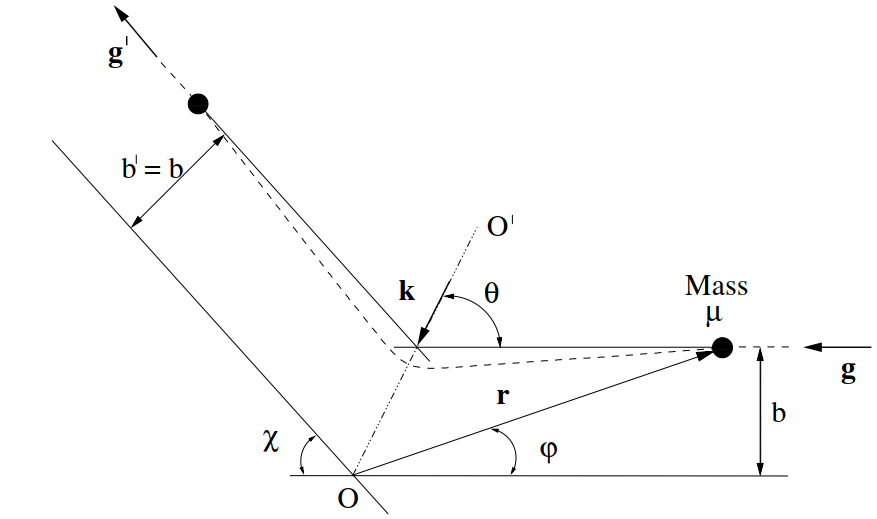
\includegraphics[scale=.5]{binary_collision}
	\caption{Kremer (2010, p. 27), Fig 1.6}
	\label{fig:binary_collision}
\end{figure}
	
	 Denote the pre- and post-collisional asymptotic velocities by $\vec{v}$, $\vec{v_1}$ and $\vec{v}'$, $\vec{v}_1'$ respectively. Define the relative pre- and post-collisional velocities, respectively, by 
\begin{equation*}
	\vec{g} = v_1 - v\, , \quad \vec{g}' = \vec{v}'-\vec{v}_1' \, .
\end{equation*}
To denote the modulus of $\vec{g}$ and $\vec{g}'$, the vector notation is dropped, e.g. $g$. $b$ denotes the offset of the centers of the molcules orthogonal to $\vec{g}$. $\varepsilon$ denotes the azimuthal angle between the two particles. 

By conservation of momentum, we have that 
\begin{equation}
\label{eq:consv_momentum}
m \vecv + m \vecv_1 = m\vecv' + m\vecv_1'\, .
\end{equation}
Equation \ref{eq:consv_momentum} yields $g' = g$. In addition, due to the hard sphere assumption, the collision is considered to be perfectly elastic, giving
\begin{equation}
\label{eq:consv_kin}
\frac{1}{2} m|\vecv| + \frac{1}{2} m|\vecv_1| = \frac{1}{2}m|\vecv'| + \frac{1}{2}m|\vecv_1'|
\end{equation}

The apsidal vector, $\vec{k}$ given by
\begin{equation*}
\vec{k} = \frac{\vec{g} - \vec{g}'}{|\vec{g} - \vec{g'}|}\, ,
\end{equation*}
bisects the angle between asymptotic relative velocities. Using this vector, we can write a relationship between the pre- and post-collisional velocities by
\begin{align*}
\vec{v}_1' &= \vec{v}_1 - \vec{k}(\vec{k} \cdot \vec{h})\, , \\
\vec{v}' &= \vec{v} + \vec{k}(\vec{k} \cdot \vec{h})\, .
\end{align*}


\section{The Boltzmann Equation}

We consider a gas enclosed in a volume. A single molecule of this gas can be described with having position $\vec{x}$ and velocity $\vec{v}$ at a time $t$. For a particular time, we can describe a molecule as being within at a single point, $(\vec{x},\vec{v})$, in 6-dmensional space known as phase space. We define the distribution function of the gas as $f(t,\vec{x},\vec{v})d\vec{x}\,d\vec{v}$ gives the number of particles within the range of $\vec{x} + d\vec{x}$ with velocities $\vec{v} + d\vec{v}$. 

In 1872 Boltzmann \cite{Boltzmann1872} introduced the Boltzmann equation which describes the time evolution of the distribution $f$. In the absence of external forces and we ignore collisions of particles, then the Boltzmann equation takes the form
\begin{equation}
\label{eq:colless_boltzmann}
\dydx{}{t}f(t, \vecx, \vecv) + \vecv \cdot \nabla_x f(t, \vecx, \vecv) = 0\, .
\end{equation}
However, when the effects of collisions cannot be neglected, the right hand side must be modified to take this into account. In this case, the Boltzmann equation takes the form of
\begin{equation}
\label{eq:boltzmann}
\dydx{}{t}f(t, \vecx, \vecv) + \vecv \cdot \nabla_x f(t, \vecx, \vecv) = I[f](t,\vecx,\vecv)\, \\ 
\end{equation}
Where $I[f]$ is referred to as the collision operator. The explicit form of $I[f]$ depends on the properties of the gas. To describe it explicitly, we make several assumptions. First, the gas composed entirely of a single species of molecule. Second, we assume hard sphere collisions as described in section \ref{sec:bincol}. 

In order to explicitly write the collision operator, we must describe the collisions within the gas. Consider a particle with velocity $\vecv$. In the volume element $\vecx d\vecx$
\begin{equation}
dt \int_{\R^3} \int_0^{b^*} \int_0^{2\pi} f_1 f b g\,  db \, d\varepsilon\, dv_1 \, dv \, .
\end{equation}

\begin{equation}
I[f](t, \vecx, \vecv) = \int_\Rexp{3} \int_\Rexp{3} (f_1' f' - f_1 f) g\, b\, db\, d\varepsilon\, d\vecv_1\, ,
\end{equation}
where,
\begin{equation*}
f_1' \equiv f(t, \vecx, \vecv_1')\quad f' \equiv f(t, \vecx, \vecv') \quad f_1 \equiv f(t, \vecx, \vecv_1 \quad f \equiv f(t, \vecx, \vecv)\, .
\end{equation*}
The Boltzmann equation is a non-linear integro-differential equation. The right hand side is a five dimensional integral that must be evaluated at each point in 6-dimensional space.

\section{Moments of the Distribution Function}

A gas is usually described by its macroscopic states. Kinetic theory defines these macroscopic properties in terms of distribution function $f(t,\vecx, \vecv)$. The first five moments of the gas are defined below.
\begin{align}
	n(t,\vec{x})&=\int_{\mathbb{R}^3}  f(t,\vec{x},\vec{v}) d\vec{v} &\text{- number density}  \label{eq:dens} \\
	\bar{v}_i(t,\vec{x})&=\frac{1}{n(t,\vec{x})} \int_{\mathbb{R}^3} m v_i f(t,\vec{x},\vec{v}) d\vec{v} &\text{- bulk velocity} \label{eq:bulk} \\
	T(t,\vec{x}) &= \frac{1}{3Rn(t,\vecx)}\int_{\mathbb{R}^3} m C^2 f(t,\vec{x},\vec{v}) d\vec{v} &\text{- temperature} \label{eq:temperature}
\end{align}
where $C_i=v_i-\bar{v}_i$, $C^2=C_1^2 + C_2^2 + C_3^2$, and $R$ is the specific gas constant. The number density $n(t, \vecx)$ denote the number of particles contained in our distribution. $\bulkv (t,\vecx)$ denotes that average velocity of particles within the gas. The temperature denotes the deviation form the average. 

An important property of the collision integral 

\section{The Maxwellian Distribution}

If the gas is free from external influence, then the gas will approach an equilibrium. In this equilibrium, the gas distribution takes a specific shape known as the Maxwellian distribution given below.
\begin{equation}
f_M(\vec{v},n,\vec{\bar{v}},T) = \frac{1}{\sqrt{2 \pi R T}^3} \exp\left( -\frac{ |\vec{v} - \vec{\bar{v}}|^2}{2RT} \right)
\end{equation} 
	
Note that the exact shape of the Maxwellian distribution depends on the macroscopic moments of the gas distribution, $n$, $\vec{\bar{v}}$, and $T$ given by equations \ref{eq:dens}, \ref{eq:bulk}, \ref{eq:temperature} respectively. This is illustrated in Figure \ref{fig:1d_maxwellian}. The distribution is centered around $\bulkv$. The temperature, $T$, controls the width of the distribution. $n$ determines the area under the curve.
\begin{figure}[h]
\centering
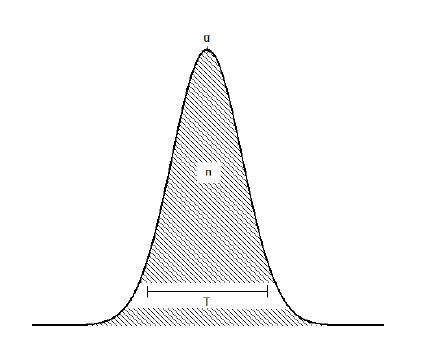
\includegraphics[scale=.5]{1D_Maxwellian}
\caption{Stolen picture need better caption}
\label{fig:1d_maxwellian}
\end{figure}

When the gas is in equilibrium, the difference between the number of particles that enter and leave a particular phase volume vanishes. In other words, 
\begin{equation*}
I[f_M](t,\vecx,\vecv) = \int_{\R^3} \int_{\R^3} f_{M1}'f_M' - f_{M1} f_M  g\, b\, db\, d\varepsilon\, d\vecv_1\ = 0
\end{equation*}

\clearpage
\addcontentsline{toc}{chapter}{References}
\begin{footnotesize}
\begin{thebibliography}{100}

\bibitem{Bird1994} G. Bird, Molecular Gas Dynamics and the Direct Simulation of Gas Flows, Clarendon Press, Oxford, 1994.

\bibitem{Boltzmann1872} L. Boltzmann, Weitere Studien u ber das Warmegleichgewicht unter Gasmolekulen. 1872.

\bibitem{Kogan1969} M. Kogan, Rarefied Gas Dynamics, Plenum Press, New York, USA, 1969.

\bibitem{Cercignani2000} C. Cercignani, Rarefied Gas Dynamics: From Basics Concepts to Actual Calculations, Cambridge University Press, Cambridge, UK, 2000.

\bibitem{Cockburn2000} B. Cockburn, G. Karniadakis, and C. Shu, Discontinuous Galerkin Methods: Theory, Computation, and Applications. Berlin: Springer, 2000.

\bibitem{Golse} F. Golse. 2006. Chapter 3 The Boltzmann Equation and Its Hydrodynamic Limits. Handbook of Differential Equations: Evolutionary Equations, 159-301.

\bibitem{AMA} A. Alekseenko, and E. Josyula: Deterministic solution of the Boltzmann equation using a discontinuous Galerkin velocity discretization. In \textit{28th International Symposium on Rarefied Gas Dynamics, 9-13 July  2012, Zaragoza, Spain, AIP Conference Proceedings,} page 8. American Institute of Physics, 2012.

\bibitem{AMA1} A. Alekseenko and E. Josyula: Deterministic solution of the spatially homogeneous Boltzmann equation using discontinuous Galerkin discretizations in the velocity space. \textit{Journal of Computational Physics,} 272(0): 170 - 188, 2014. 

\bibitem{Struchtrup2005} H. Struchtrup, Macroscopic Transport Equations for Rarefied Gas Flows Approximation Methods in Kinetic Theory, Interaction of Mechanics and Mathematics Series, Springer, Heidelberg, 2005.

\bibitem{Worner} S. Worner, "Fast Fourier Transform," Swiss Federal Institute of Technology Zurich, Zurich.

\bibitem{Osgood2007} B. Osgood, "N-dimensional Fourier Transform." The Fourier Transform and Its Applications. Stanford U, 2007. 428. Print.

\bibitem{Bethune2010} I. Bethune, OpenMP Implementation of Fast Fourier Transform. Digital image. FFT. 14 Sept. 2010.

%Read More: http://www.worldscientific.com/doi/abs/10.1142/S0218202591000137

\bibitem{KALMAN} D. Kalman, A Singularly Valuable Decomposition: The SVD of a Matrix. \textit{The College Mathematics Journal,} The American University, Washington, DC (2002).

\bibitem{LAPACK} E Anderson, Z. Bai, C. Bischof, S. Blackford, J. Demmel, J. Dongarra, J. Du Croz, A. Greenbaum, S. Hammarling, A. McKenne and D. Sorensen, \textit{LAPACK Users' Guide, Third Edition, 1999, pub. Society for Industrial and Applied Mathematics, Philadelphia, PA, ISBN 0-89871-447-8}.

\bibitem{PROPACK} R. Larsen Computing the Singular Value Decomposition of Large and Sparse or Structured Matrices. Computer software. PROPACK. Vers. 2.1. N.p., 20 Apr. 2005.

\bibitem{Burden2004} L. Burden, and J. Douglas Faires, Numerical Analysis. 8th ed. Boston: PWS-Kent Pub., 2004.

\bibitem{INVTRANSF} L. Devroye, "Inversion by Numerical Solution of F(X) = U." New York: Springer-Verlag, 1986.

\bibitem{EMA} I. Dinov, "Statistics Online Computational Resource." SOCR. eScholarship Repository, University of California, 2008.

\bibitem{GAMBA} Gamba, Irene M., and Chenglong Zhang. "A Conservative Discontinuous Galerkin Scheme with $O(N^2)$ Operations in Computing Boltzmann Collision Weight Matrix." (2014)

\bibitem{GAMBA1} I. M. Gamba and S. H. Tharkabhushanam. Shock and Boundary Structure Formation by Spectral-Lagrangian Methods for the Inhomogeneous Boltzmann Transport Equation. \textit{Journal of Computational Mathematics}, 2010.

\bibitem{GAMBA2} Irene M. Gamba and Sri Harsha Tharkabhushanam. Spectral-lagrangian methods for collisional models of non-equilibrium statistical states. \textit{J. Comput. Phys.,} 228(6):2012-2036, April 2009.

%% The followings are from the actual paper:

\bibitem{ANDALLAH} L. Andallah and H. Babovsky. A discrete Bolzmann equation based on a cub-octahedron in $\R^3$. \textit{SIAM Journal on Scientific Computing,} 31(2):799-825, 2009.

\bibitem{ARISTOV1} V. V. Aristov and S. A. Zabelok. A deterministic method for the solution of the Boltzmann equation with parallel computations. \textit{Zhurnal Vychislitel'noi Tekhniki i Matematicheskoi Physiki,} 42(3):425-437, 2002.

\bibitem{ARISTOV2} V. V. Aristov. \textit{Direct Methods for Solving the Boltzmann Equation and Study of Nonequilibrium Flows.} Fluid Mechanics and Its Application. Kluwer Academic Publishers, 2001.

\bibitem{BABOVSKY} Hans Babovsky. Kinetic models on orthogonal groups and the simulation of the Bolzmann Equation. \textit{AIP Conference Proceedingds,} 1084(1), 2008.

\bibitem{BHATNAGAR} P. L. Bhatnagar, E. P. Gross, and M. Krook. A model for collision processes in gases. i. small amplitude processes in charged and neutral one-component systems. \textit{Phys. Rev.,} 94(3):511-525, May 1954.

\bibitem{BIRD} G. A. Bird. \textit{Molecular Gas Dynamics and the Direct Simulation of Gas Flows.} Oxford Engineering Science Series. Oxford University Press, New York, USA, 1994.

\bibitem{BOYD} Iain D Boyd. \textit{Vectorization of a Monte Carlo simulation scheme for nonequilibrium gas dynamics. Journal of Computational Physics,} 96(2):411-427, 1991.

\bibitem{FILBET} F. Filbet, C. Mouhot, and L. Pareschi. Solving the Bolzmann equation in n log2n. \textit{SIAM Journal on Scientific Computing,} 28(3):1029-1053, 2006.

\bibitem{FOX} R. O. Fox and P. Vedula. Quadrature-based moment model for moderately dense polydisperse gas-particle flows. \textit{Industrial and Engineering Chemistry Research,} 49(11):5174-5187, 2010.

\bibitem{GREEN} B. I. Green and P. Vedula. Validiation of a collisional lattice Boltzmann method. In \textit{20th AIAA Computational Fluid Dynamics Conference, 27-30 June 2011, Honolulu Hawaii,} number 3403 in AIP Conference Proceedings, page 14. American Institute of Physics, 2011.

\bibitem{HOLWAY} L. H. Holway. New statistical models for kinetic theory: methods of construction. \textit{Phys. Fluids,} 9(9):1658-1673, 1966.

\bibitem{KIRSCH} R. Kirsch and S. Rjasanov. A weak formulation of the Boltzmann equation based on the Fourier transform. \textit{Journal of Statistical Physics,} 129(3):483-492, 2007.

\bibitem{LEVERMORE} C. David Levermore. Moment closure hierarchies for kinetic theories. \textit{Journal of Statistical Physics,} 83(5-6
:1021-1065, 1996.

\bibitem{MAJORANA} Armando Majorana. A numerical model of the Boltzmann equation related to the discontinuous Galerkin method. \textit{Kinetic and Related Models,} 4(1):139-151, 2011.

\bibitem{MOUHOT} Clement Mouhot and Lorenzo Pareschi. Fast algorithms for computing the Boltzmann collision operator. \textit{Mathematics of Computation,} 75(256):PP. 1833-1852, 2006.

\bibitem{PANFEROV} Vladislav A. Panferov and Alexei G. Heintz. A new consistent discrete-velocity model for the Boltzmann equation. \textit{Mathematical Methods in the Applied Sciences,} 25(7):571-593, 2002.

\bibitem{PARESCHI} Lorenzo Pareschi and Benoit Perthame. A Fourier spectral method for homogeneous Boltzmann equations. \textit{Trnasport Theory and Statistical Physics,} 25(3-5):369-382, 1996.

\bibitem{SCHROCK} C. R. Schrock and A. W. Wood. Convergence of a distributional Monte Carlo method for the Boltzmann equation. \textit{Advances in Applied Mathematics and Mechanics,} 4(1):102-121, 2012.

\bibitem{SCHROCK1} C. R. Schrock and A. W. Wood. Distributional Monte Carlo technique for rarefied gas dynamics. \textit{Journal of Thermophysics and Heat Transfer,} 26(1)185-189, 2012.

\bibitem{SELDEN} NATHANIEL SELDEN, CEDRICK NGALANDE, NATALIA GIMELSHEIN, SERGEY GIMELSHEIN, and ANDREW KETSDEVER. Origins of radiometric forces on a circular vane with a temperature gradient. \textit{Journal of Fluid Mechanics,} 634:419-431, 9 2009.

\bibitem{SHAKHOV} E. M. Shakhov. Approximate kinetic equations in rarefied gas theory. \textit{Fluid Dynamics,} 3(1):112-115, 1968

\bibitem{SHAKHOV1} E. M. Shakhov. Generalization of the krook kinetic relaxation equation. \textit{Fluid Dynamics,} 3(5):95-96, 1968.

\bibitem{TITAREV} V. A. Titarev. Efficient deterministic modeling of three dimensional rarefied gas flows. \textit{Communications in the Computational Physics,} 162(1):162-192, 2012.

\bibitem{SUCCI} S. Succi. \textit{The Lattice Boltzmann Equation: For Fluid Dynamics and Beyond.} Numerical Mathematics and Scientific Computation. Clarendon Press, 2011.

\bibitem{TCHEREMISSINE} F. G. Tcheremissine. SOlution to the Boltzmann kinetic equation for high-speed flows. \textit{Computational Mathematics and Mathematical Physics,} 46(2):315-329, 2006.
 
\end{thebibliography} 
\end{footnotesize}

\end{document}